\documentclass[10pt,a4paper]{article}
% for margining standards
\usepackage[left=3cm,right=3cm,top=3cm,bottom=3cm]{geometry}
% for counting references as a section
\usepackage[numbib,notlof,notlot,nottoc]{tocbibind}
% useful packages
\usepackage{
                graphicx, setspace, fontspec, caption,
                subcaption, float, polyglossia, rotating,
                lscape, pdflscape, indentfirst, tocloft,
                multirow, mathtools, currfile
            }
% paragraph related package
\usepackage[parfill]{parskip}
% use bzar font(THIS MUST BE LOADED BEFORE XePerian PACKAGE)
\setmainfont{BZar.ttf}
% the dear XePersian package
\usepackage{xepersian}
%
% General settings goes here.
%
% lines space
\renewcommand{\baselinestretch}{1.5}
% paragraph first line indention
\setlength{\parindent}{1cm}
% paragraph spacing
\setlength{\parskip}{1em}
% set graphics' path
\graphicspath{ {images/} }
% make table of content dotted
\renewcommand{\cftsecleader}{\cftdotfill{\cftdotsep}}
% define a new command as {half-space} in english
\newcommand{\halfspace}{\hspace{0pt}}
% define a new command as {half-space} in persian
\newcommand{\نیمفاصله}{\halfspace}
% define a shortcut for half-space in general
\renewcommand{\ }{\halfspace}
% define a new command for ease of use for rendering reference
\newcommand{\renderref}[1] { \begingroup \let\clearpage\relax \include{#1} \endgroup }
\newcommand{\مق}{\lr}
\newcommand{\fig}[4]{\begin{figure}%
\centering%
\includegraphics[width=#2\textwidth]{#1}%
\caption{#3}\label{#4}%
\end{figure}}
%
% DOCUMENT BEGIN
%
\begin{document}
\title{گزارش تمرین سوم
\\
طبقه\ بندی تصاویر با استفاده از\\
\lr{Convolutional Neural Network} و \lr{GoogleNet}
}
\author{داریوش حسن\ پور آده}
\date{۹۳۰۸۱۶۴}
\maketitle
\قسمت{قسمت ۱}
بنده ۶ عکس از محیط اطراف گرفتم را به شبکه دادم و نتایج\ اش به صورت زیر بدست آمد.\بند
\begin{figure}[h!]
\centering
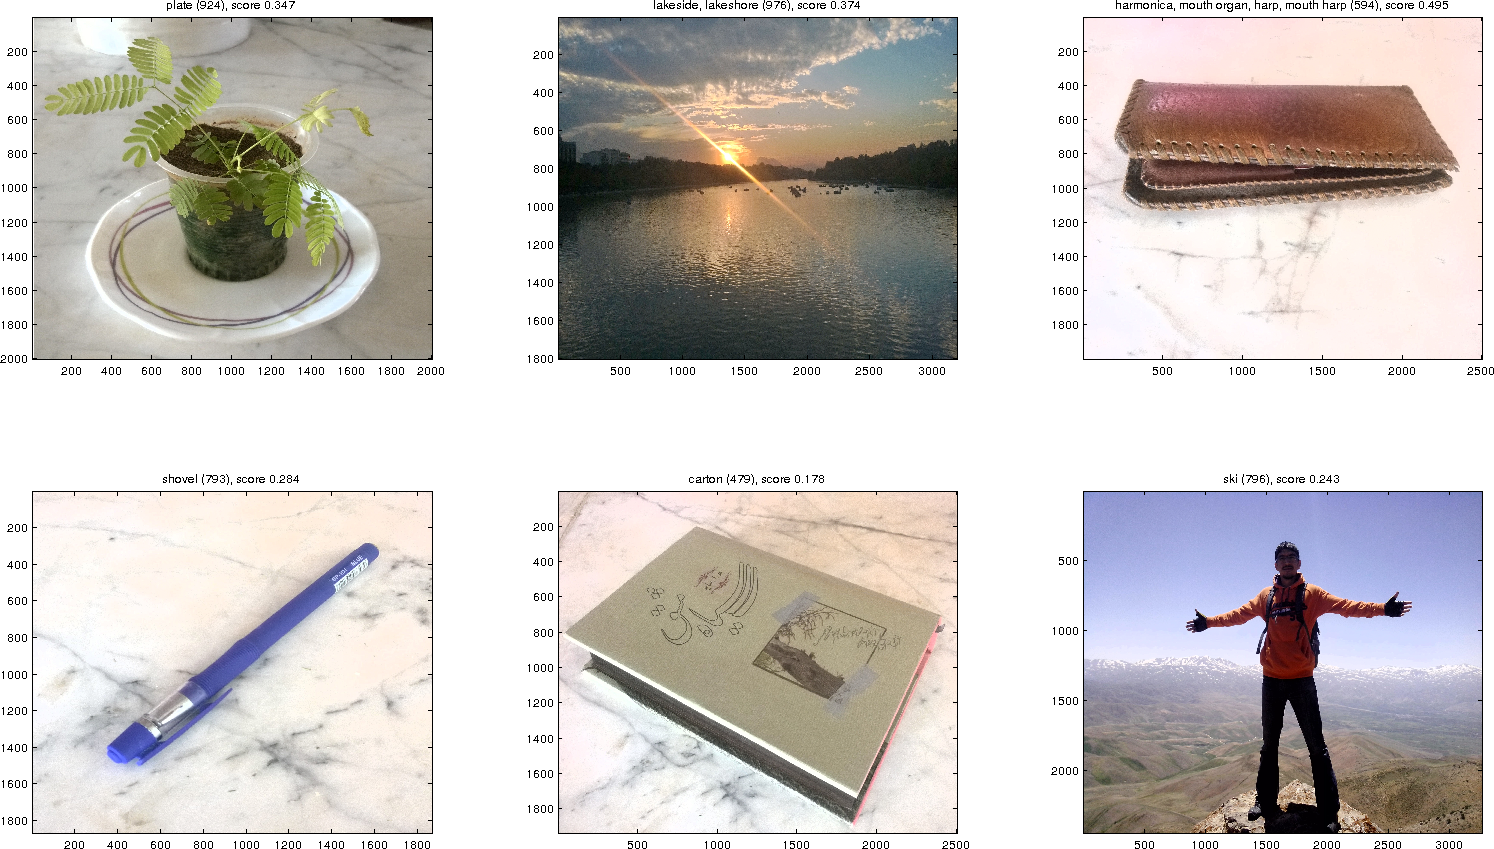
\includegraphics[width=\textwidth]{../sec_A/results/results}
\end{figure}
 که عکس اول(ردیف بالا، سمت راست) مربوط به «کیف پول» بنده می\ باشد که شبکه «سازدهنی» طبقه\ بندی است، عکس دوم مربوط که غروب خورشید که روی پل سی\ وسی پل گرفته شده است، که شبکه «دریاچه» طبقه\ بندی کرده است. عکس سوم مربوط به گیاهی است که در یک داخل یک زیراستکانی قرار داده شده است، که شبکه «بشقاب» طبقه\ بندی کرده است، عکس چهارم(ردیف پایین، سمت راست) مربوط به عکس بنده در ارتفاعات کوه\ ها می\ باشد، که شبکه «آسمان» طبقه\ بندی کرده است، عکس چهارم مربوط که به یک کتاب شعر از «هوشنگ ابتهاج» می\ باشد که شبکه «مقوا» طبقه\ بندی کرده است و آخر مربوط به یک عدد خودکار می\ باشد که شبکه «بیل» طبقه\ بندی کرده است.  همان\ طور که می\ بینیم به جز عکس آخر(خودکار) در مابقی عکس\ ها آنچه که شبکه طبقه\ بندی کرده است با آنچه که عکس\ ها بودند چندان هم بی\ ربط نیست، که نشان از خوب کار کردن شبکه\ ی \مق{GoogleNet} می\ باشد.
\قسمت{قسمت ۲}
در این قسمت عکس\ هایی که برای طبقه\ بندی در نظر گرفته است، عکس\ های \مق{MRI} مربوط به «مغز»\زیرنویس{۶۲ عدد عکس} و «زانو»\زیرنویس{۸۰ عدد عکس} می\ باشد که از موتور جستجوگر گوگل جمع\ آوری شده\ اند. همان\ طور که خواسته شده است ۸۰٪ از داده به صورت تصادفی به عنوان داده\ های آموزشی و ۲۰٪ مابقی را به عنوان داده\ های تست در نظر گرفته شدند. نتایج هر ۳ قسمت تکلیف در شکل زیر آمده است.
\begin{figure}[h!]
\centering
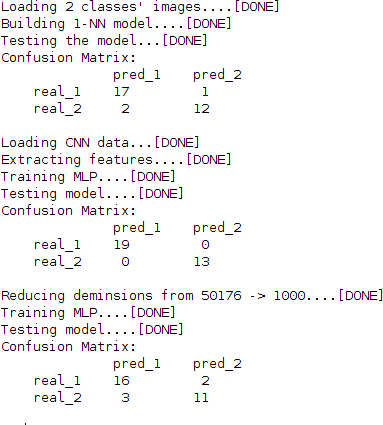
\includegraphics[scale=.8]{../sec_B/results/results}
\end{figure}
همان\ طور که در شکل بالا مشاهده می\ شود به ازای هر زیرقسمت(یعنی آموزش و ساخت مدل توسط «نزدیک\ ترین همسایه\زیرنویس{\مق{K-NN where K = 1}}»، استفاده از گوگل\ نت به عنوان استخراج کننده\ ی ویژگی و یک شبکه\ ی چندلایه و استفاده از \مق{‌PCA} و یک شبکه\ ی چندلایه) داده\ های تست را با استفاده از مدل بدست آمده تست کرده و \مق{Confusion Matrix} آن را رسم کرده\ ایم. برای اینکه بتوانیم نتایج حاصل از \مق{PCA} را با نتایج حاصل از گوگل\ نت مقایسه کنیم به تبعیت از ساختار شبکه\ ی گوگل\ نت عکس\ ها را از یک بردار ۵۰,۱۷۶ به یک بردار ۱۰۰۰ تایی کاهش دادیم و سپس توسط یک شبکه\ ی
$1000 \times 30 \times 1$
آموزش دادیم(همین ترکیب شبکه برای قسمت ۲.۲ تکلیف نیز در نظر گرفته شده است.). همان\ طور که می\ بینیم شبکه\ ای که با توسط گوگل\ نت کاهش بعد داده شده است بدون خطا همه\ ی داده\ های تست را به درستی طبقه\ بندی کرده است در حالی که هم در نزدیک\ ترین همسایه و هم در \مق{PCA} خطای طبقه\ بندی مشاهده می\ شود؛ که نشان می\ دهد گوگل\ نت می\ تواند کاهش\ بعد دهنده\ ی خوبی باشد.\بند
خروجی شبکه\ ی چندلایه در هردو قسمت ۲.۱ و ۲.۲ یک نورون بوده که برای کلاس یکی از دسته عکس\ ها مقدار هدف ۰ درنظر گرفته شده و برای دیگری ۱، در خروجی شبکه اگر بیشتر از ۰.۵ باشد ۱ در نظر گرفته می\ شود و اگر کمتر از ۰.۵ باشد ۰ در نظر گرفته می\ شود. در «نزدیک\ ترین همسایه» ۹٪ خطا، در «کاهش بعد با گوگل\ نت» ۰٪ خطا و در «کاهش بعد با \مق{PCA}» ۱۵٪ خطا داشته\ ایم، همان\ طور که می\ بینیم «کاهش\ بعد توسط گوگل\ نت و طبقه\ بندی توسط \مق{MLP}» حتی از «نزدیک\ ترین همسایه» نیز بهتر عمل کرده است.
\قسمت{قسمت ۳}
در این قسمت بنده عکس\ ها را دانلود کرده و برچسب\ های عکس\ های مرتبط با هر یک از عکس\ ها را استخراج کرده و سعی در ایجاد شبکه\ ای کانولشنی که بتواند بروی داده\ ها یادگیری انجام دهد کردم، متاسفانه نسخه\ ی \مق{beta17} کتابخانه\ ی \مق{MatConvnet} مشکل داشت و بخاطر این موضوع بود که در نسخه\ ی ابتدایی این تکلیف که بنده قبل از ۱۳ دی آپلود کردم مشکل عدم توانایی ایجاد شبکه\ ای جهت یادگیری داده\ ها را گزارش کردم\زیرنویس{علت بارگذاری زودتر این تکلیف بخاطر این بود که دکتر صفایانی در ابتدا تاریخ ۱۳ را به عنوان آخرین مهلت بارگذاری تکلیف اعلام کرده بودند و بعد از چند روز بعد از بارگذاری تکلیف توسط بنده اعلام شد که مهلت ارائه\ ی تکلیف به ۳۰ دی ماه تغییر یافت!} که بعد از تغییر نسخه\ ی کتابخانه به \مق{beta16} مشکل گزارش شده برطرف شد؛ از آنجایی که هیچ\ گونه مستند رسمی جهت چگونگی آموزش شبکه توسط این کتابخانه منتشر نشده است، به ناچار از مهندسی معکوس مثال\ های موجود در فایل\ های کتابخانه استفاده شد تا بتوانم شبکه را بنویسم. ظاهرا به باید داده\ های ورودی شبکه در قابل یک ساختار با فرمت مشخص به تابع یادگیری \مق{cnn\_train}\زیرنویس{که این تابع را نیز مثال\ های موجود در کتابخانه استخراج کردم در کنار کدها ارسال نموده\ ام.} ارسال شود که بنده مشابه کدهای آنچه که در مثال برای بارگذاری داده\ های \مق{mnist} آورده شده است برای بارگذاری داده\ های \مق{Jaffe} کدهایی نوشتم.\بند
در حالت خلاصه بنده از تابع \مق{cnn\_train} موجود در میان مثال\ های کتابخانه جهت آموزش شبکه\ ی کانولوشن استفاده کردم، تابع \مق{getImdb} که وظیفه\ ی بارگذاری داده\ ها به فرمتی که سازگار با تابع \مق{cnn\_train} باشد را با مهندسی معکوس مثال\ های موجود در کتابخانه نوشتم و در نهایت یک اسکریپت جهت اجرای قسمت سوم نوشته شده است.\بند
بنده با استفاده از ۳ لایه\ ی کانولشنی و ۲ عدد لایه\ ی \مق{max-pooling} توانستم در نهایت به دقت ۹۸٪ بروی داده\ های ارزیابی\زیرنویس{Validation Set} با معیار \مق{Top-1} برسم و با معیار \مق{Top-5} به دقت ۱۰۰٪ رسیدم و برای داده\ های آموزشی میزان دقت با هر دو معیار ۱۰۰٪ بوده است، البته لازم به ذکر است که معیار \مق{Top-5} در این تکلیف با این دیتاست خاص که کلا ۶ کلاس دارد به درد نمی\ خورد و اطلاع بدرد بخوری از میزان خوبی عملکرد شبکه به ما نمی\ دهد(زیرا کلا ۶ کلاس داریم.). بطور خلاصه توضیح در مورد دو میعار گفته شده(یعنی \مق{Top-1} و \مق{Top-5}) می\ توان گفت که برای اولین بار توسط \مق{Krizhevskym et al.}\
\cite{krizhevsky2012imagenet}
ارائه شد. معیار \مق{Top-1} به این معنی است که در صورتی که کلاس واقعی نمونه\ ای با کلاسی که خروجی شبکه به عنوان بیشترین و محتمل\ ترین کلاس آن نمونه پیش\ ببینی می\ کند برابر باشد می\ گوییم که شبکه درست تشخیص داده است و یکی شمارنده تشخیص درست اضافه میکنیم و در نهایت آن شمارنده را به تعداد نمونه\ ها تقسیم می\ کنیم که میزان دقت شبکه می\ شود؛ معیار \مق{Top-5} نیز همانند \مق{Top-1} می\ باشد با این تفاوت که در صورت که کلاس نمونه جز ۵ محتمل\ ترین کلاسی که شبکه برای آن نمونه تشخیص داده باشد، باشد آنگاه به شمارنده\ ی صحت شبکه یکی اضافه کرده و در نهایت به تعداد کل تقسیم می\ کنیم.\بند
برای آموزش شبکه عکس\ های مرتبط با هر کلاس را که توسط پوشه\ ها جدا شده\ اند بارگذاری میکنیم و به طور تصادفی ۸۰٪ از این داده\ ها را به عنوان داده\ های آموزشی و ۲۰٪ مابقی به عنوان داده\ های تست انتخاب می\ کنیم به شبکه می\ دهیم. برای آموزش شبکه از تکنیک \مق{mini-batch} با سایز ۴۰ استفاده کردم. تعداد اپوک\ ها ۱۰۰ و ضریب یادگیری ۰.۰۰۱ در نظر گرفته شده است. با استفاده از داده\ های آموزشی و تست استخراج شده شبکه را ۵ بار آموزش داده و در بعد از اتمام هر سری آموزش نتایج را ذخیره کرده و دوباره به آموزش شبکه با وزن\ دهی\ های اولیه جدید می\ پردازیم، این کار را ۵ بار طبق دستورالعمل ارائه شده در تکلیف انجام می\ دهیم. نتایج اجرای هر سری را در محل\ های جداگانه ذخیره میکنیم که در در شکل\ های
\ref{fig:epoch1}-\ref{fig:epoch5}
آمده است. همانطور که گفته شد معیار \مق{Top-5} برای داده\ های آموزشی این تکلیف که کلا ۶ کلاس دارد معیار به درد بخوری نیست لذا از اینجا به بعد منظور از «میزان دقت» همان میزان دقت با استفاده از معیار \مق{Top-1} می\ باشد. همان\ طور که مشاهده می\ شود شبکه اجرای خوبی بروی داده\ ها دارد و کمترین دقت ۹۴.۵٪ و بیشترین دقت ۱۰۰٪ را داشته است. در شکل\ های
\ref{fig:avg_mean} و \ref{fig:avg_obj}
میانگین این ۵ اجرا را در نموداری آورده شده است که بطور میانگین شبکه در نهایت دقت ۹۷.۳٪ را میزان انرژی ۰.۰۱ بروی داده\ های آموزشی و ۰.۱۳ بروی داده\ های تست دارد.\بند
همان\ طور که مشاهده می\ کنیم نتایج اجرای شبکه\ ی کانولوشن رضایت بخش بوده است و در نتایج با وجود اینکه افت و خیزی مشاهده می\ کنیم ولی در نهایت به یک دقت خوبی همگرا می\ شود. داده\ های نتایج و شبکه\ ی هر اجرا به همرا کدها ارسال گردیده است.
\begin{figure}
\centering
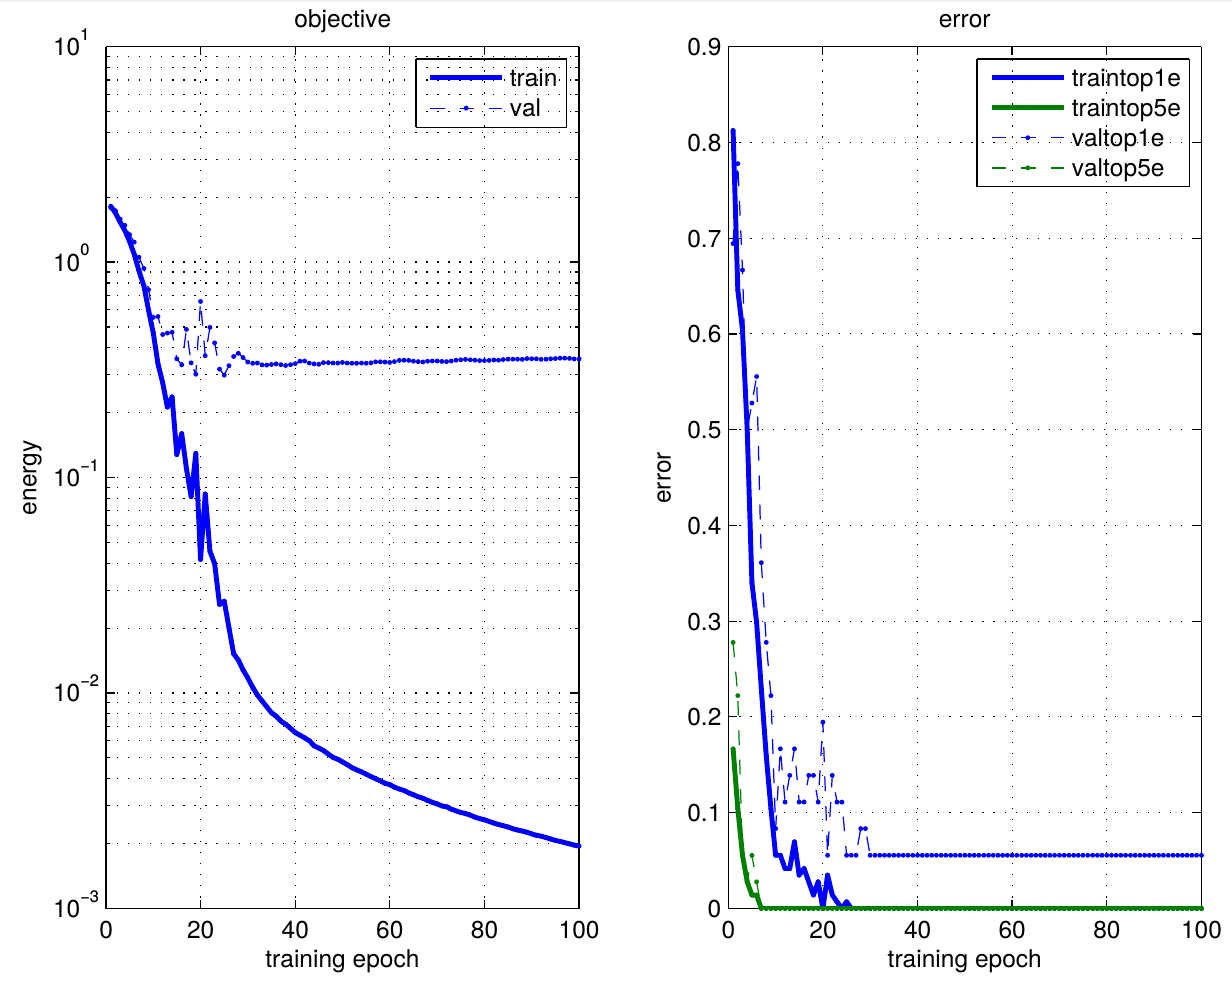
\includegraphics[width=.8\textwidth]{../sec_C/results/1.png}
\caption{نتیجه\ ی اجرای ۵/۱، دقت بروی داده\ های تست: ۹۴.۵٪ انرژی شبکه بروی داده\ های تست: ۰.۳۵}\label{fig:epoch1}
\end{figure}
\begin{figure}
\centering
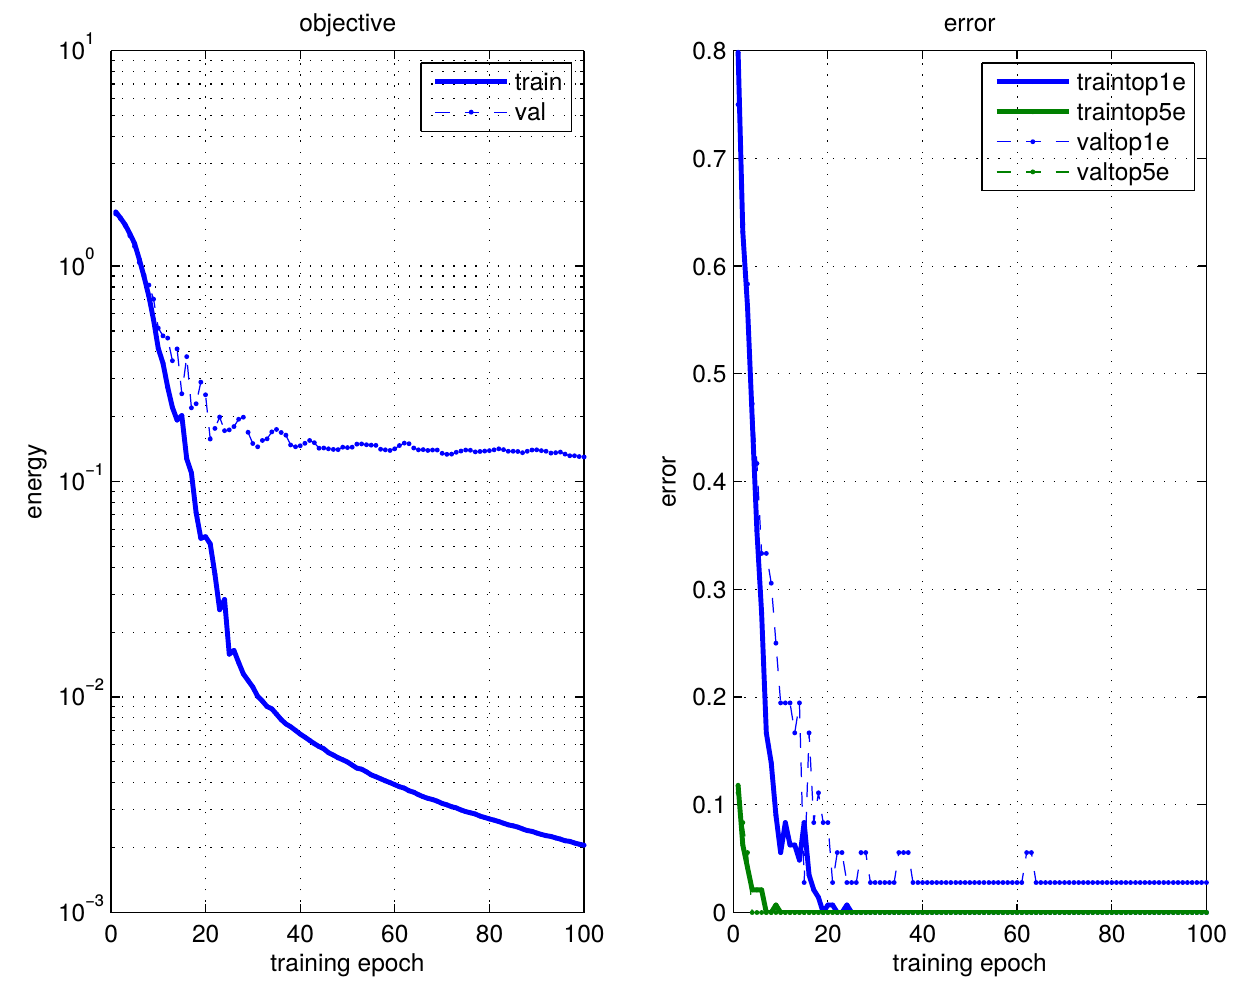
\includegraphics[width=.8\textwidth]{../sec_C/results/2.png}
\caption{نتیجه\ ی اجرای ۵/۲، دقت بروی داده\ های تست: ۹۷.۲٪ انرژی شبکه بروی داده\ های تست: ۰.۱۲}\label{fig:epoch2}
\end{figure}
\begin{figure}
\centering
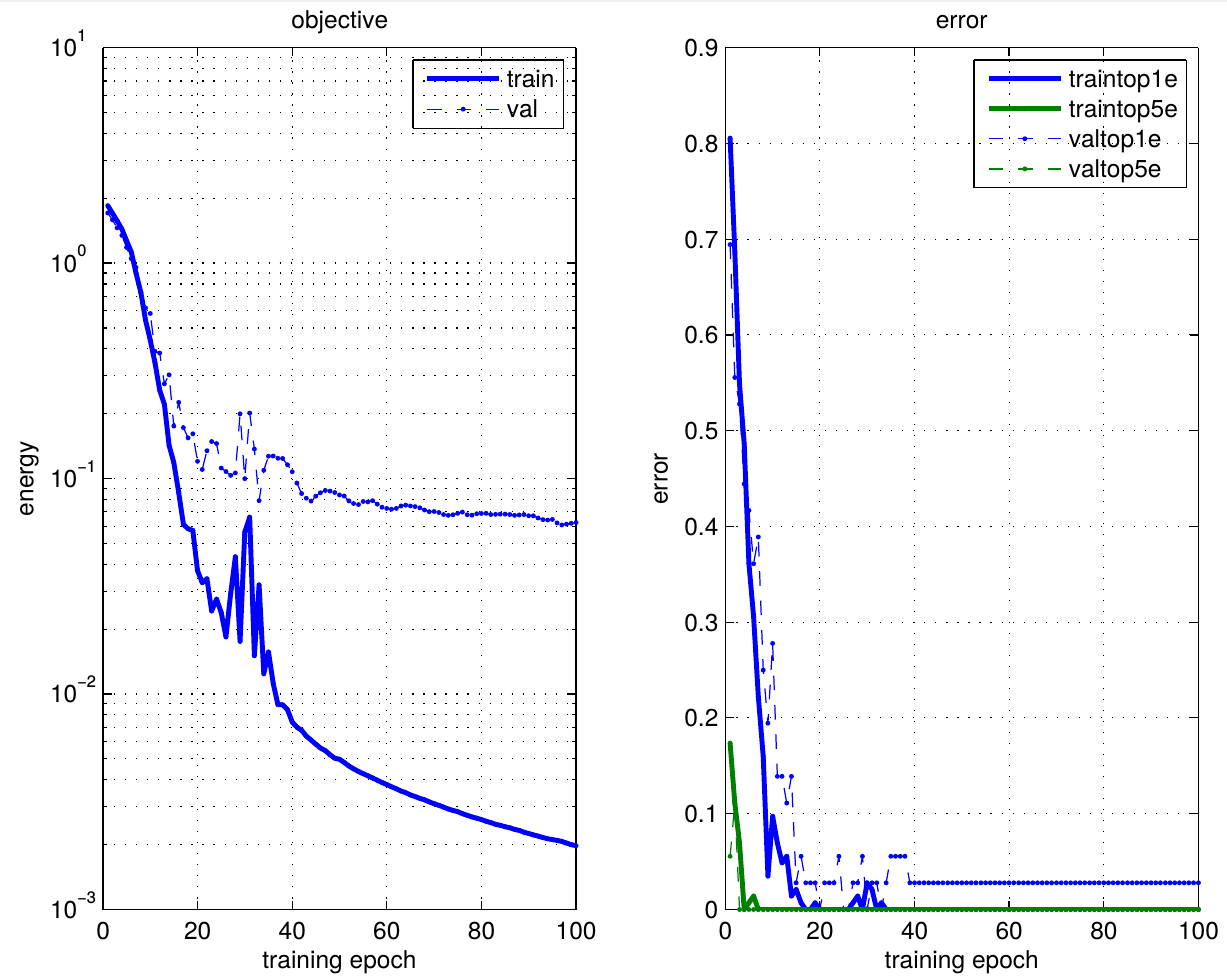
\includegraphics[width=.8\textwidth]{../sec_C/results/3.png}
\caption{نتیجه\ ی اجرای ۵/۳، دقت بروی داده\ های تست: ۹۷.۲٪ انرژی شبکه بروی داده\ های تست: ۰.۰۶}\label{fig:epoch3}
\end{figure}
\begin{figure}
\centering
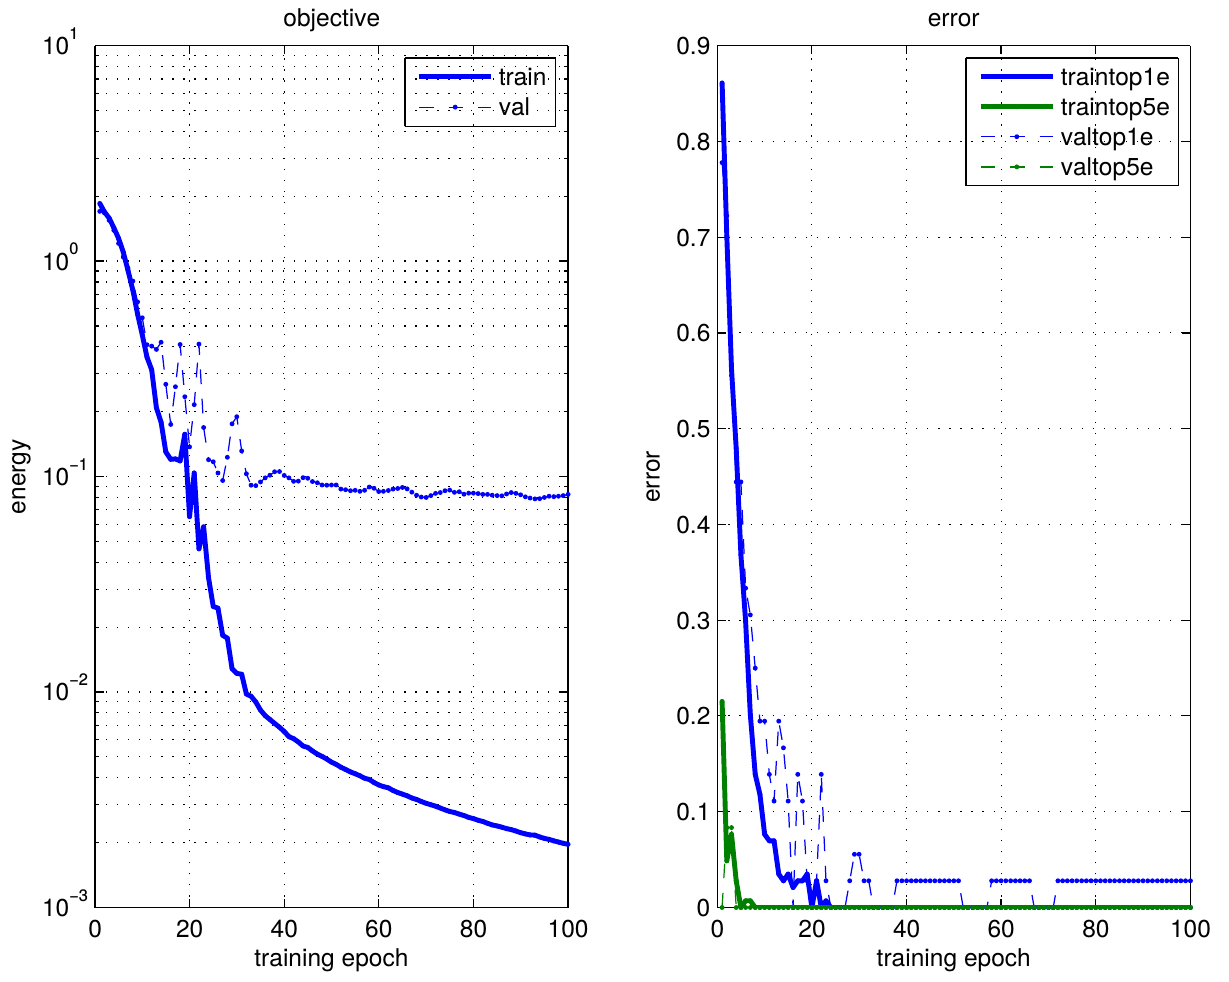
\includegraphics[width=.8\textwidth]{../sec_C/results/4.png}
\caption{نتیجه\ ی اجرای ۵/۴، دقت بروی داده\ های تست: ۹۷.۲٪ انرژی شبکه بروی داده\ های تست: ۰.۰۸}\label{fig:epoch4}
\end{figure}
\begin{figure}
\centering
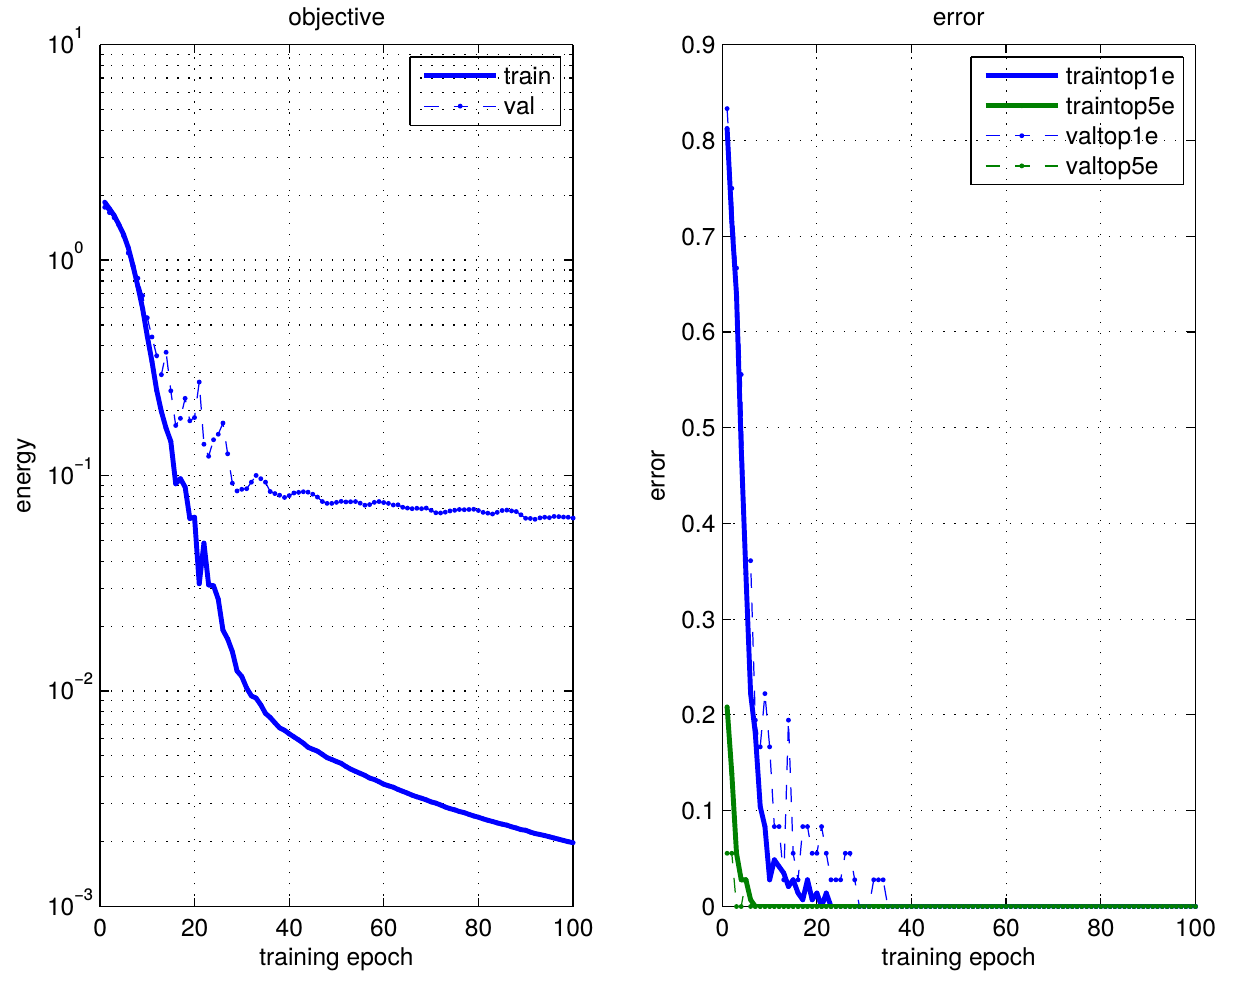
\includegraphics[width=.8\textwidth]{../sec_C/results/5.png}
\caption{نتیجه\ ی اجرای ۵/۵، دقت بروی داده\ های تست:۱۰۰٪ انرژی شبکه بروی داده\ های تست: ۰.۰۶}\label{fig:epoch5}
\end{figure}
\begin{figure}
\centering
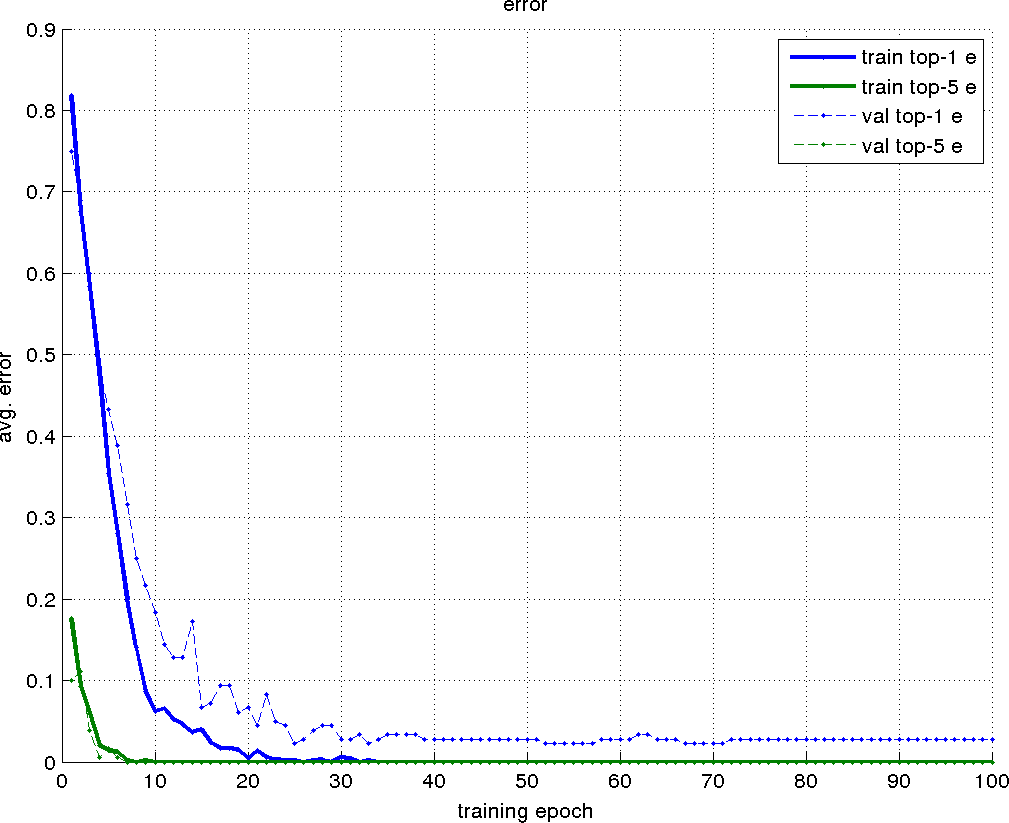
\includegraphics[width=.8\textwidth]{../sec_C/results/error.png}
\caption{میانگین خطا ۵ اجرا به ازای ۱۰۰ اپوک}\label{fig:avg_mean}
\end{figure}
\begin{figure}
\centering
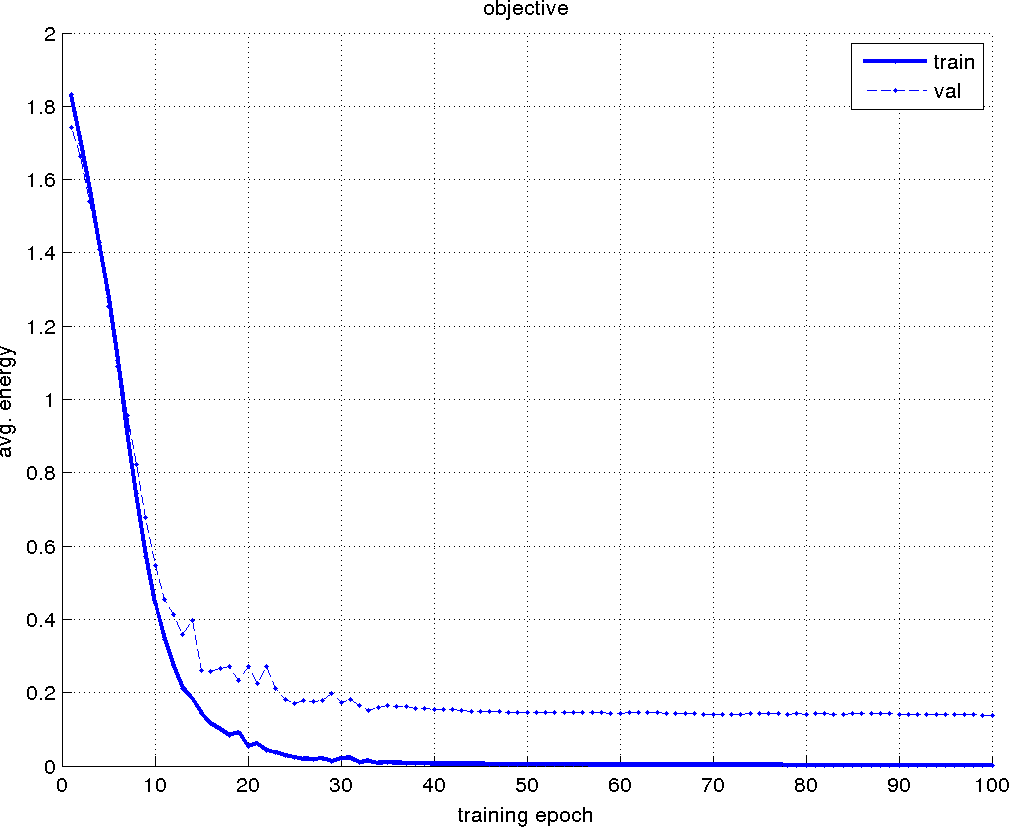
\includegraphics[width=.8\textwidth]{../sec_C/results/obj.png}
\caption{میانگین انرژی ۵ اجرا به ازای ۱۰۰ اپوک}\label{fig:avg_obj}
\end{figure}
\begin{figure}
\centering
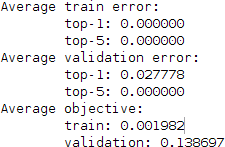
\includegraphics[width=.4\textwidth]{../sec_C/results/texts.png}
\caption{جمع\ بندی کلی از نتایج اجراها}
\end{figure}

\قسمت*{مراجع}
\renderref{reference}
\end{document}
